\chapter{Анализ графов спутников полученных при помощи polaris 2.0}

Для оценки влияния космической погоды на бортовые системы и целевую аппаратуру
малых космических аппаратов (МКА) в этой главе будет проведен комплексный анализ
зависимости параметров телеметрии \cite{green_2017_impact}
\cite{schlag_2018_numerical} \cite{boumghar_2018_enhanced}, индексов солнечной
активности и геомагнитных индексов. В основе исследования лежит применение
модели машинного обучения Polaris ML. Результаты работы модели будут
представлены в виде двухмерного графа связности, отражающего выявленные
взаимосвязи между исследуемыми параметрами.

Для расчета и анализа графа связности будет использована обширная база данных
телеметрии сети наземных станций SatNOGS. Параметры солнечной активности будут
извлечены из следующих основных источников:

\begin{itemize}
	\item Центр прогнозирования космической погоды (Space Weather Prediction Center, SWPC/SWO) \cite{swpc_noaa_data_souce};
	\item Центр наблюдения и анализа данных о влиянии Солнца в Брюсселе (Solar Influences Data Analysis Center, S.I.D.C.) \cite{silso_snd_data_source};
	\item Канадская радиоастрофизическая обсерватория в Пентиктоне \cite{swgc_flux_data_source}.
\end{itemize}

Далее представлена таблица \ref{tab:detailed_solar_geo_params} с основными анализируемыми параметрами солнечной активности

\begin{longtable}{|l|p{12cm}|}
	\caption{Подробное описание параметров солнечной и геомагнитной активности}
	\label{tab:detailed_solar_geo_params}                                                                                                                                                                                                                                                                                                                                                                                                                                                                                                    \\

	\hline
	\textbf{Параметр}     & \textbf{Описание}                                                                                                                                                                                                                                                                                                                                                                                                                                                                                                \\
	\hline
	\endfirsthead

	\multicolumn{2}{c}%
	{\tablename\ \thetable\ -- \textit{Продолжение}}                                                                                                                                                                                                                                                                                                                                                                                                                                                                                         \\
	\hline
	\textbf{Параметр}     & \textbf{Описание}                                                                                                                                                                                                                                                                                                                                                                                                                                                                                                \\
	\hline
	\endhead

	\hline
	\multicolumn{2}{|r|}{\textit{Продолжение на следующей странице}}                                                                                                                                                                                                                                                                                                                                                                                                                                                                         \\
	\hline
	\endfoot

	\hline
	\endlastfoot

	ssn                   & Среднемесячное число солнечных пятен — ключевой индикатор солнечной активности, получаемый Центром наблюдения и анализа данных о влиянии Солнца в Брюселе (S.I.D.C.). Солнечные пятна представляют собой области с пониженной температурой, вызванные магнитными полями, которые препятствуют конвективным процессам. Их количество варьируется в зависимости от 11-летнего цикла солнечной активности, что делает ssn важным параметром для понимания солнечного поведения и его влияния на космическую погоду. \\
	\hline
	smoothed\_ssn         & Сглаженное число солнечных пятен — это усредненное значение количества солнечных пятен за определенный период, также предоставляемое S.I.D.C. Сглаживание позволяет устранить краткосрочные колебания и выявить долгосрочные тенденции в солнечной активности, что критически важно для прогноза космической погоды и оценки воздействия на Землю.                                                                                                                                                               \\
	\hline
	observed\_swpc\_ssn   & Среднемесячное число солнечных пятен, зарегистрированное Центром прогнозирования космической погоды (SWPC/SWO). Этот параметр служит основой для оценки текущего состояния солнечной активности и ее потенциального влияния на магнитосферу Земли, что имеет значение для защиты спутников и других технологий.                                                                                                                                                                                                  \\
	\hline
	smoothed\_swpc\_ssn   & Сглаженное число солнечных пятен, полученное из наблюдений SWPC/SWO. Оно позволяет анализировать долгосрочные изменения в солнечной активности, что особенно полезно для научных исследований и разработки моделей предсказания космической погоды.                                                                                                                                                                                                                                                              \\
	\hline
	f10.7                 & Среднемесячные значения потока радиоизлучения на длине волны 10,7 см — важный индикатор солнечной активности, измеряемый канадской радиоастрофизической обсерваторией в Пентиктоне, Британская Колумбия. Этот параметр коррелирует с количеством солнечных пятен и служит основным показателем для оценки интенсивности радиоволн, излучаемых Солнцем.                                                                                                                                                           \\
	\hline
	smoothed\_f10.7       & Сглаженные значения потока радиоизлучения 10,7 см, которые помогают устранить кратковременные колебания и выявить более стабильные тренды в солнечной радиации, что имеет критическое значение для исследований климатических изменений и космической погоды.                                                                                                                                                                                                                                                    \\
	\hline
	observed flux         & Наблюдаемое значение солнечного излучения — это интегральная мера выбросов энергии от Солнца, полученная с помощью радиотелескопов. Это значение подвержено модуляции двумя основными факторами: уровнем солнечной активности и изменением расстояния между Землей и Солнцем, что делает его важным для понимания динамики солнечного излучения и его воздействия на земную атмосферу.                                                                                                                           \\
	\hline
	adjusted flux         & Наблюдаемое значение солнечного излучения, скорректированное на изменения расстояния между Землей и Солнцем и данное для среднего расстояния.                                                                                                                                                                                                                                                                                                                                                                    \\
	\hline
	Fredericksburg A      & Индекс магнитной активности в районе Фредериксбурга (США). Используется для мониторинга геомагнитных изменений. Представляет собой линейную шкалу, отражающую амплитуду возмущений магнитного поля Земли. Единица измерения: нанотесла (нТл). Диапазон значений: от 0 до 400 нТл.                                                                                                                                                                                                                                \\
	\hline
	Fredericksburg K 0-3  & Категории магнитной активности K-индекса (низкий уровень, 0-3) в Фредериксбурге. K-индекс измеряется каждые три часа и отражает локальные геомагнитные возмущения. Безразмерная величина. Соответствует возмущениям до 20 нТл.                                                                                                                                                                                                                                                                                   \\
	\hline
	Fredericksburg K 3-6  & Категории магнитной активности K-индекса (умеренный уровень, 3-6) в Фредериксбурге. Указывает на усиление геомагнитной активности. Безразмерная величина. Соответствует возмущениям от 20 до 120 нТл.                                                                                                                                                                                                                                                                                                            \\
	\hline
	Fredericksburg K 6-9  & Категории магнитной активности K-индекса (высокий уровень, 6-9) в Фредериксбурге. Свидетельствует о сильных геомагнитных возмущениях. Безразмерная величина. Соответствует возмущениям от 120 до 300 нТл и выше.                                                                                                                                                                                                                                                                                                 \\
	\hline
	fluxcarrington        & Номер периода вращения Каррингтона для корреляции солнечного излучения. Используется для отслеживания солнечных явлений, связанных с вращением Солнца. Безразмерная величина. Период Каррингтона $\approx$ 27.2753 дня.                                                                                                                                                                                                                                                                                          \\
	\hline
	fluxobsflux           & Наблюдаемый поток радиоизлучения (10.7 см) на момент измерения. Измеряется в солнечных единицах потока (с.е.п., 1 с.е.п. = \(10^{-22}\) Вт·м\(^{-2}\)·Гц\(^{-1}\)). Является важным индикатором солнечной активности.                                                                                                                                                                                                                                                                                            \\
	\hline
	fluxadjflux           & Приведенный поток радиоизлучения (с поправкой на расстояние между Землей и Солнцем). Позволяет сравнивать данные, полученные в разные периоды года. Единица измерения: с.е.п.                                                                                                                                                                                                                                                                                                                                    \\
	\hline
	fluxursi              & Поток URSI, принятый стандарт в радиофизике для солнечного радиоизлучения. Обеспечивает стандартизированное измерение солнечного радиопотока. Единица измерения: с.е.п.                                                                                                                                                                                                                                                                                                                                          \\
	\hline
	SNvalue (hemispheric) & Наблюдаемое число солнечных пятен по полушариям. Важный показатель солнечной активности, отражающий асимметрию активности Солнца. Безразмерная величина.                                                                                                                                                                                                                                                                                                                                                         \\
	\hline
	SNerror (hemispheric) & Ошибка в оценке числа солнечных пятен по полушариям. Указывает на точность измерений и возможные погрешности. Безразмерная величина.                                                                                                                                                                                                                                                                                                                                                                             \\
	\hline
	Nb\_observations      & Количество наблюдений, использованных для вычисления параметров. Важно для оценки статистической значимости данных. Целое число.                                                                                                                                                                                                                                                                                                                                                                                 \\
\end{longtable}


Далее будут представлены графы кросс-корреляций между инженерными и внешними параметрами спутников Каждый узел графа соответствует телеметрическому или внешнему параметру, рёбра отражают наличие статистически значимой корреляции, а цвет рёбер - силу связи (от синего - слабая, фиолетовый - среднее, красный - сильная).


\section{Структурный анализ графов кросс-корреляций для спутника GRIFEX}

\subsection{Положение задачи}

Для спутника GRIFEX, выполненного с применением радиационно-стойких материалов и
современной архитектуры, построение графов кросс-корреляций позволяет выявить не
только прямое влияние солнечной активности на параметры аппаратуры, но и оценить
устойчивость систем к внешним воздействиям. На рисунках~\ref{fig:grifex_dgd},
\ref{fig:grifex_flux}, \ref{fig:grifex_hemi}, \ref{fig:grifex_ssn} приведены
графы кросс-корреляций между основными параметрами, характеризующими как
солнечную, так и геомагнитную активность.

\begin{figure}[H]
	\centering
	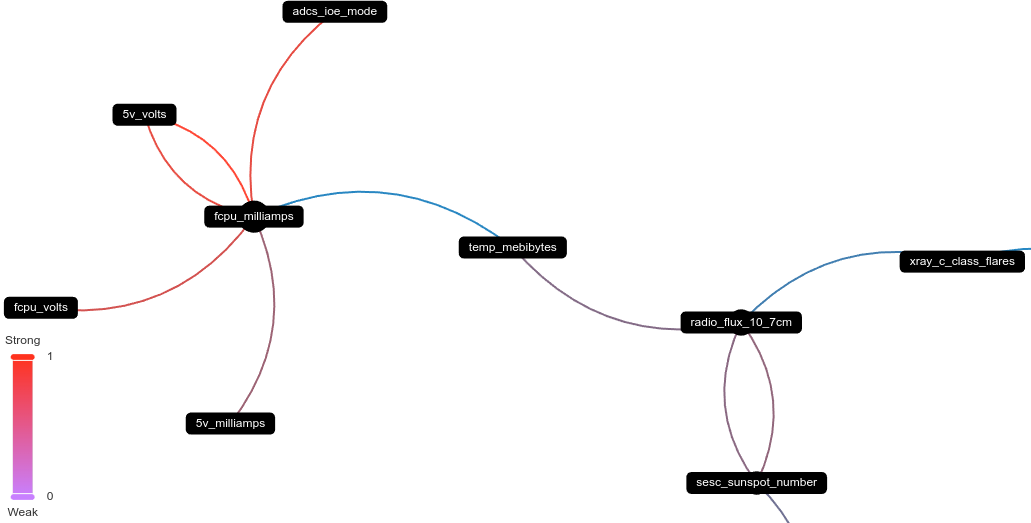
\includegraphics[width=0.95\textwidth]{sat/grifex_dgd.png}
	\caption{Граф кросс-корреляций для основных солнечных и геомагнитных индексов (GRIFEX)}
	\label{fig:grifex_dgd}
\end{figure}

\begin{figure}[H]
	\centering
	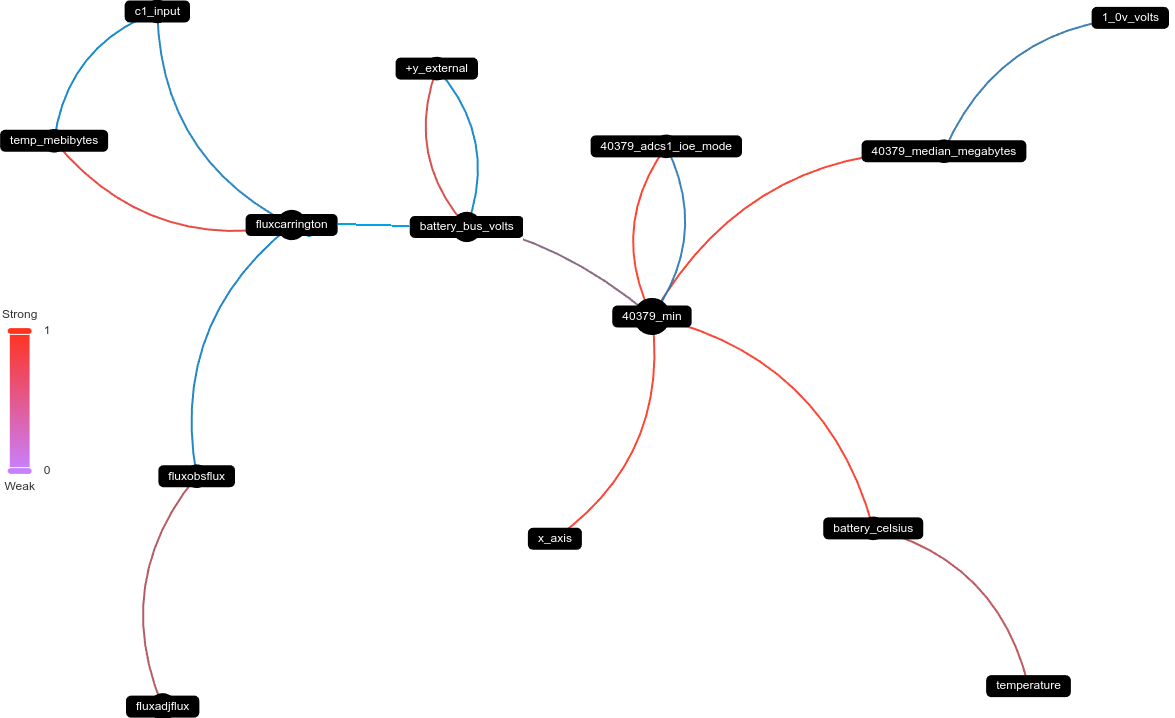
\includegraphics[width=0.95\textwidth]{sat/grifex_flux.png}
	\caption{Граф кросс-корреляций по потокам солнечного радиоизлучения (GRIFEX)}
	\label{fig:grifex_flux}
\end{figure}

\begin{figure}[H]
	\centering
	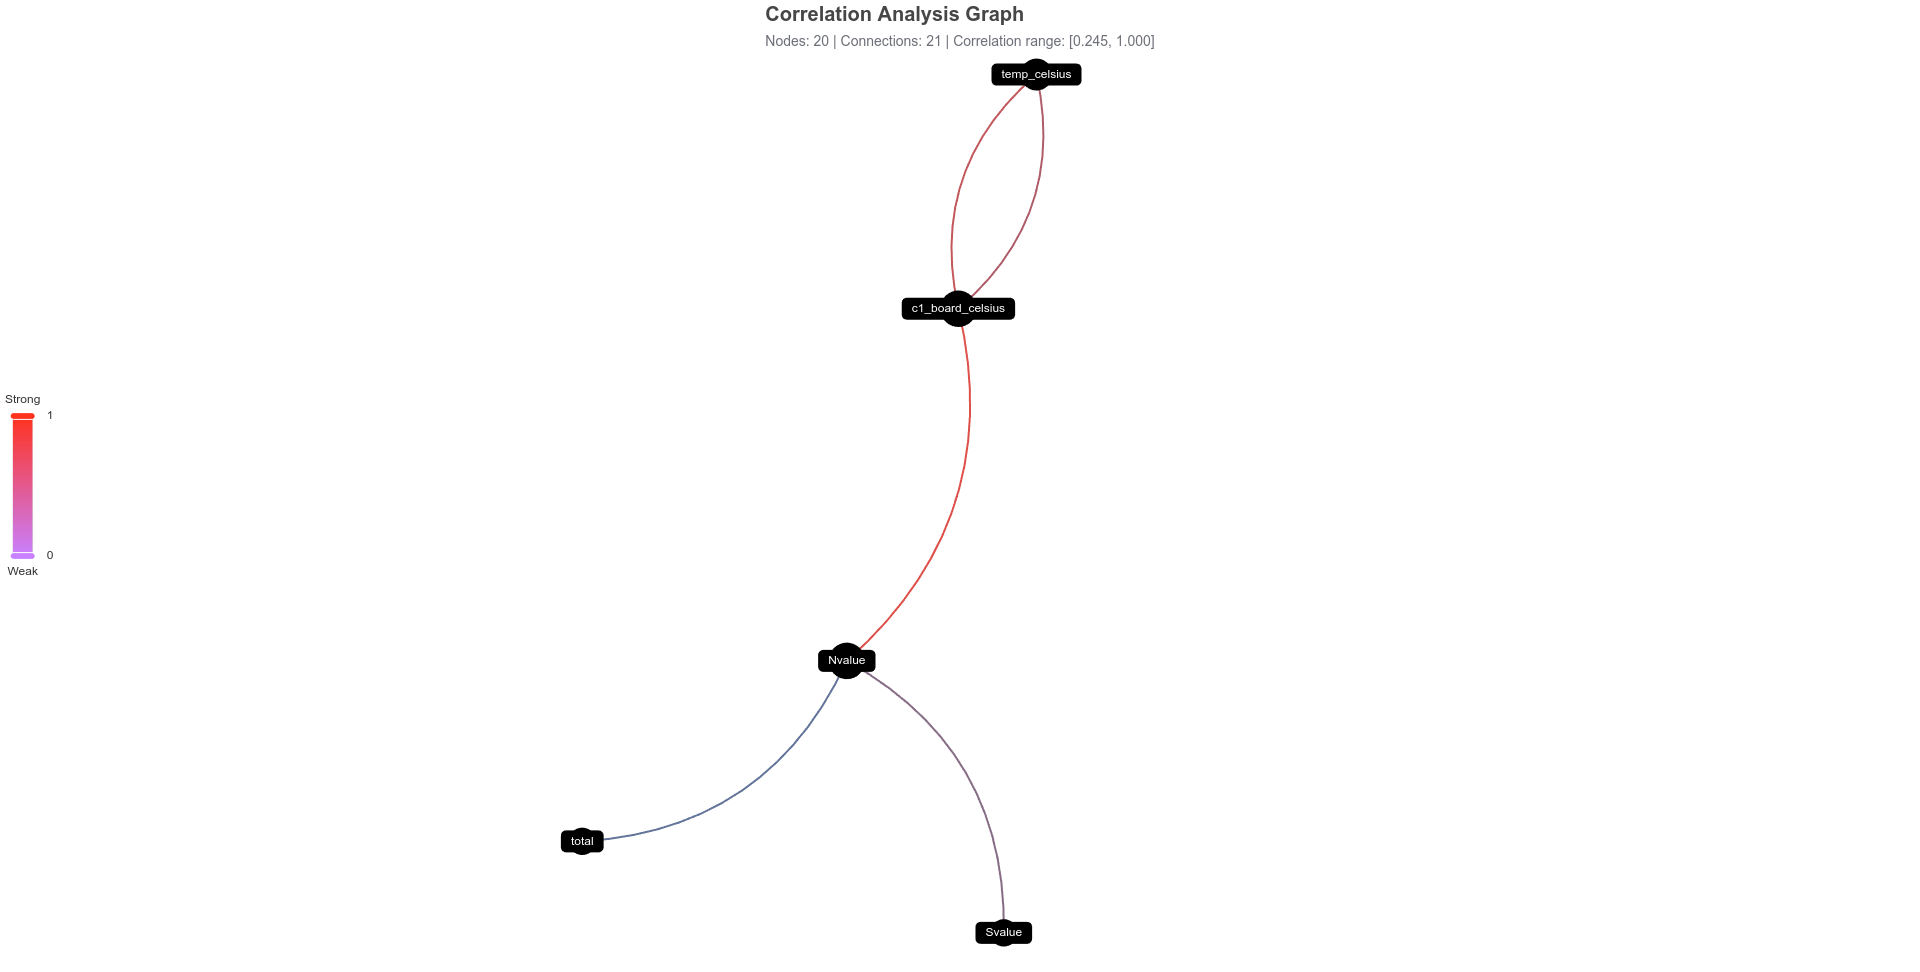
\includegraphics[width=0.95\textwidth]{sat/grifex_hemi.png}
	\caption{Граф кросс-корреляций по параметрам солнечных пятен по полушариям (GRIFEX)}
	\label{fig:grifex_hemi}
\end{figure}

\begin{figure}[H]
	\centering
	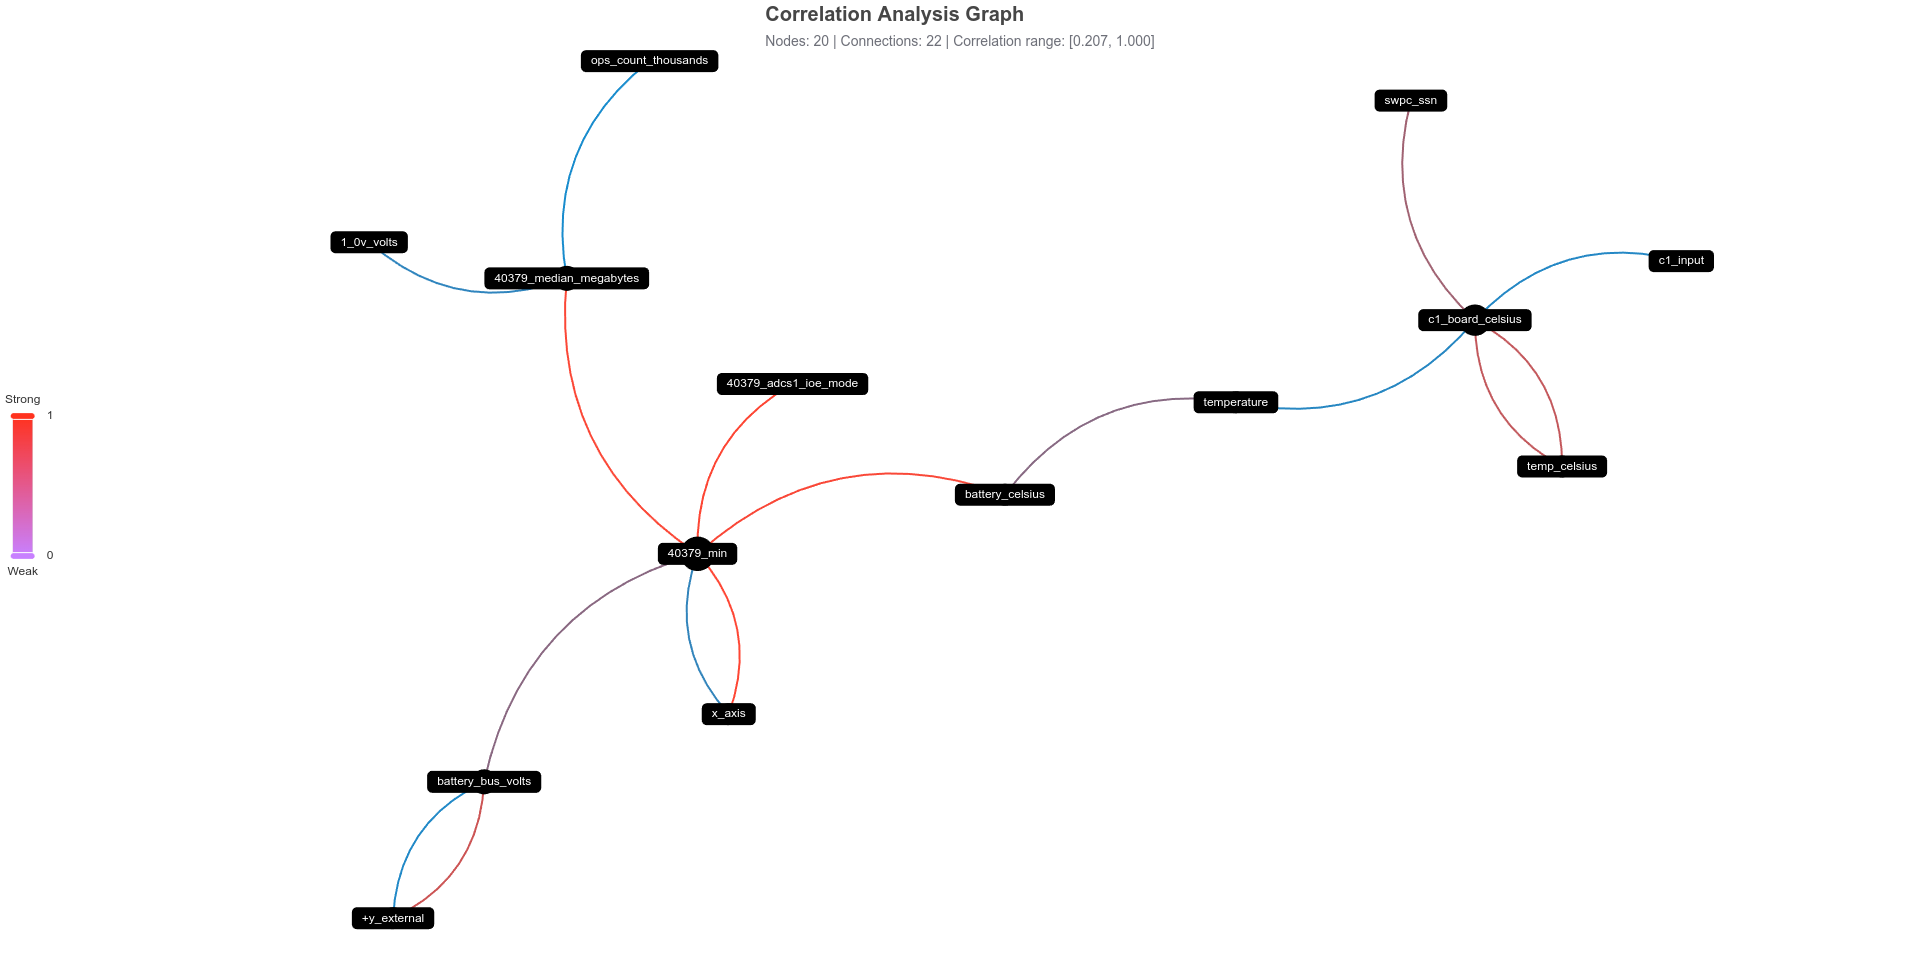
\includegraphics[width=0.95\textwidth]{sat/grifex_ssn.png}
	\caption{Граф кросс-корреляций по числу солнечных пятен (GRIFEX)}
	\label{fig:grifex_ssn}
\end{figure}

\subsection{Структурный анализ и физическая трактовка связей}

Анализируя структуру графов, можно отметить, что наибольшая плотность и сила
связей наблюдается между однородными параметрами солнечной активности, такими
как среднемесячное число солнечных пятен (\texttt{ssn}), сглаженное число пятен
(\texttt{smoothed\_ssn}), а также различные версии наблюдаемых и сглаженных
данных по числу пятен (\texttt{observed\_swpc\_ssn},
\texttt{smoothed\_swpc\_ssn}). Это объясняется тем, что все перечисленные
параметры отражают одну и ту же физическую сущность - магнитную активность на
поверхности Солнца, проявляющуюся в виде пятен, и различаются лишь методикой
усреднения и источником данных~\cite{sidc_manual}.

Потоки радиоизлучения (\texttt{f10.7}, \texttt{fluxobsflux},
\texttt{fluxadjflux}, \texttt{fluxursi}) также образуют тесно связанный кластер.
Данные параметры измеряются на длине волны 10,7 см и служат стандартом для
оценки уровня ультрафиолетового и рентгеновского излучения Солнца, оказывающего
непосредственное влияние на ионосферу и, как следствие, на работу радиосистем
спутника~\cite{f107_standard}. Сильные корреляции внутри этого кластера
подтверждают физическую однородность процессов генерации радиоизлучения на
Солнце.

В отличие от солнечных параметров, геомагнитные индексы (\texttt{Fredericksburg
	A}, \texttt{Fredericksburg K 0-3}, \texttt{K 3-6}, \texttt{K 6-9}) демонстрируют
более слабые и разреженные связи с солнечными показателями. Это связано с тем,
что геомагнитная активность - результат сложного взаимодействия солнечного ветра
и магнитосферы Земли, где задержки и нелинейные эффекты существенно ослабляют
прямую корреляцию~\cite{geomag_handbook}. Тем не менее, при анализе временных
рядов можно наблюдать, что периоды высокой солнечной активности (рост числа
пятен и потока F10.7) приводят к увеличению числа магнитных бурь и, как
следствие, к росту значений геомагнитных индексов.

Особый интерес представляет влияние солнечной активности на технические
параметры спутника GRIFEX. В отличие от большинства спутников класса CubeSat,
GRIFEX построен с применением инновационных архитектурных и технологических
решений, ориентированных на работу в условиях повышенного радиационного фона и
экстремальных температурных колебаний. Ключевой особенностью является
использование гибридного фокального модуля (FPA), в котором кремниевые
SiPIN-диоды, произведённые Raytheon Vision Systems, интегрированы с современной
БИС-схемой (ROIC) с аналогово-цифровыми преобразователями в каждом
пикселе~\cite{norton2012spaceborne, eoportal_grifex}. Это решение обеспечивает
не только высокую помехоустойчивость, но и устойчивость к радиационным
воздействиям, что нетипично для стандартных CubeSat, традиционно использующих
коммерческие компоненты без специальной защиты.

Вся система управления и обработки данных построена на базе FPGA Xilinx
Virtex-5, что позволило реализовать отказоустойчивую архитектуру с минимизацией
числа точек отказа и резервированием ключевых функций~\cite{eoportal_grifex}.
Для GRIFEX были специально выбраны компоненты с повышенной радиационной
стойкостью: это касается как цифровых, так и аналоговых трактов. По данным MXL,
в конструкцию включены дополнительные экранирующие элементы, а также реализованы
алгоритмы коррекции ошибок памяти и мониторинга питания~\cite{mxl_grifex}.

Такой подход позволил существенно снизить количество сбоев и перезагрузок
аппаратуры даже в периоды экстремальных солнечных событий, что подтверждается
инженерными телеметрическими данными за весь период
эксплуатации~\cite{mxl_grifex}. В частности, при увеличении солнечной активности
наблюдается рост выработки энергии солнечными панелями, что приводит к повышению
токов и напряжений на бортовых шинах. Это, в свою очередь, способствует
поддержанию стабильной работы вычислительных блоков и уменьшению числа аварийных
перезапусков. Таким образом, положительное влияние солнечной активности
проявляется в увеличении энергетического ресурса спутника, при условии
эффективной защиты от радиационных воздействий.

На графах кросс-корреляций это выражается в виде сильных связей между
параметрами, характеризующими солнечную активность и электрические показатели
(ток, напряжение, температура панелей). В периоды низкой солнечной активности,
наоборот, возможно снижение выработки энергии, что увеличивает риск сбоев и
требует применения дополнительных мер энергосбережения.

\subsection{Заключение}

Структурный анализ графов кросс-корреляций для спутника GRIFEX позволяет сделать
следующие выводы. Во-первых, высокая степень корреляции между однородными
солнечными параметрами подтверждает корректность и согласованность используемых
методик измерения. Во-вторых, относительно слабая связь между солнечными и
геомагнитными индексами обусловлена сложностью процессов передачи солнечного
воздействия через магнитосферу Земли. В-третьих, применение радиационно-стойких
материалов и архитектурных решений обеспечивает устойчивость аппаратуры к
солнечным вспышкам, а увеличение солнечной активности, как правило, приводит к
росту энергетических возможностей и снижению числа сбоев.

\section{Структурный анализ графов кросс-корреляций и особенностей спутника ENSO}

\subsection{Структурные и технологические особенности спутника ENSO}

ENSO (\textit{Expleo Nanosat for Solar-irradiance Observations}) - это
исследовательский 1U CubeSat, разработанный компанией Expleo совместно с
Университетским космическим центром Монпелье (CSUM) для задач мониторинга
солнечной активности и её влияния на ионосферу~\cite{expleo_enso_pdf,
	nanosats_enso, expleo_enso_launch}. Масса спутника составляет около 1 кг,
габариты - 10$\times$10$\times$10 см. ENSO оснащён развертываемой шестиметровой
антенной для передачи высокочастотного сигнала на наземные станции SANSA в
Антарктиде, а также камерой для вторичных задач сбора
данных~\cite{nanosats_enso, expleo_enso_launch}.

Конструкция спутника выполнена по классической схеме CubeSat: основной силовой
набор и панели изготовлены из алюминиевого сплава с анодированием для повышения
коррозионной стойкости и минимизации дегазации~\cite{expleo_enso_pdf,
	nanosats_enso}. Внутренние элементы электроники и крепежа используют стандартные
полимерные материалы, такие как полиимид (Kapton) для изоляции и защиты от
температурных перепадов, а также фторполимеры для кабельных
соединений~\cite{curbell_plastics}. Вся компонентная база построена на
коммерческих элементах (COTS), что характерно для современных малых спутников,
ориентированных на минимизацию стоимости и времени
разработки~\cite{expleo_enso_pdf, nanosats_enso}.

В отличие от специализированных радиационно-стойких платформ, в ENSO не
применяются rad-hard компоненты: устойчивость к космическим воздействиям
достигается за счёт оптимизации орбиты (низкая околоземная, минимизация времени
пребывания в радиационных поясах), базового экранирования алюминиевыми стенками
(толщина порядка 1–2 мм, что соответствует типичным рекомендациям NASA для
CubeSat~\cite{nasa_shielding}), а также программных методов коррекции ошибок
передачи и хранения данных~\cite{expleo_enso_pdf, nanosats_enso,
	nasa_shielding}. В ходе наземных испытаний ENSO прошёл тестирование на вибрации
и термовакуум, подтверждена работоспособность в диапазоне температур от –40°C до
+50°C в выключенном состоянии и от –20°C до +40°C в рабочем
режиме~\cite{expleo_enso_pdf}.

Таким образом, ENSO - типичный представитель NewSpace-подхода: лёгкая,
компактная платформа с минимальной массой, построенная на коммерческих
компонентах, с базовой защитой от радиации и температурных воздействий,
рассчитанная на ограниченный срок службы (до 4 лет) в условиях низкой
околоземной орбиты. Основная уязвимость - чувствительность к солнечным вспышкам
и радиационным событиям, что компенсируется резервированием каналов передачи и
программной устойчивостью~\cite{nasa_shielding, expleo_enso_pdf}.

\subsection{Структурный анализ}

В данном разделе рассматривается спутник ENSO, для которого построены графы
кросс-корреляций между инженерными и внешними параметрами
(рис.~\ref{fig:enso_sunspot}, \ref{fig:enso_ssn}, \ref{fig:enso_flux}). Для ENSO
проведён углублённый анализ структуры, особенностей используемых материалов и
архитектурных решений, а также рассмотрено влияние солнечной активности на
функционирование его систем.

\begin{figure}[H]
	\centering
	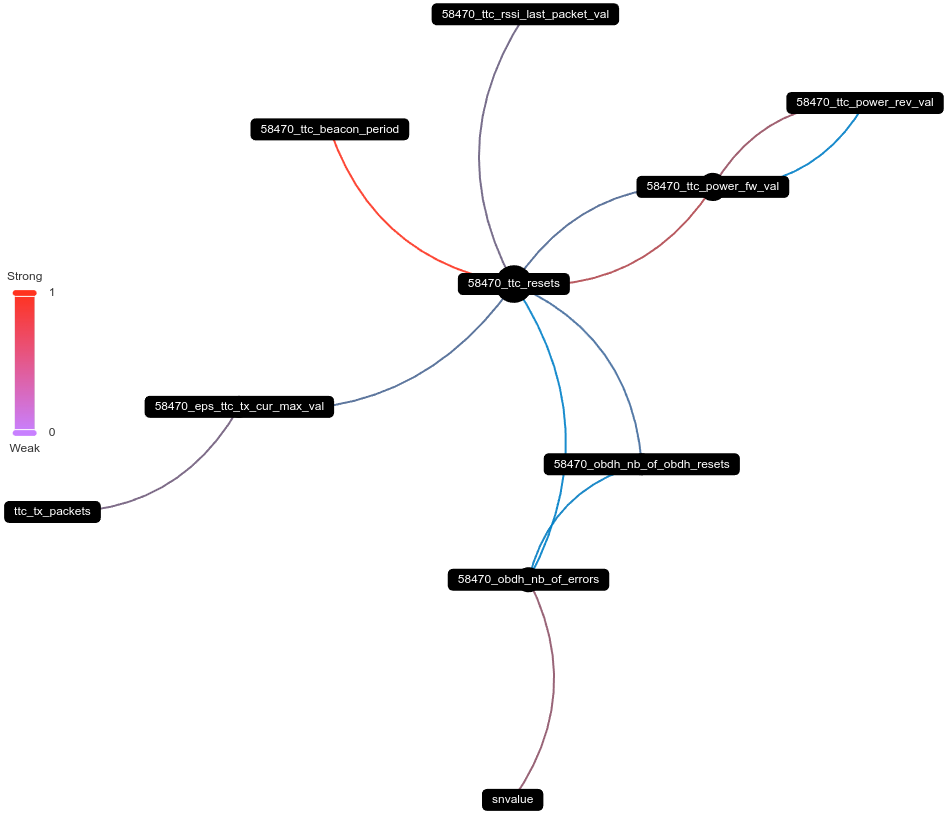
\includegraphics[width=0.95\textwidth]{sat/enso_sunspot.png}
	\caption{Граф кросс-корреляций по солнечным пятнам и инженерным параметрам (ENSO)}
	\label{fig:enso_sunspot}
\end{figure}

\begin{figure}[H]
	\centering
	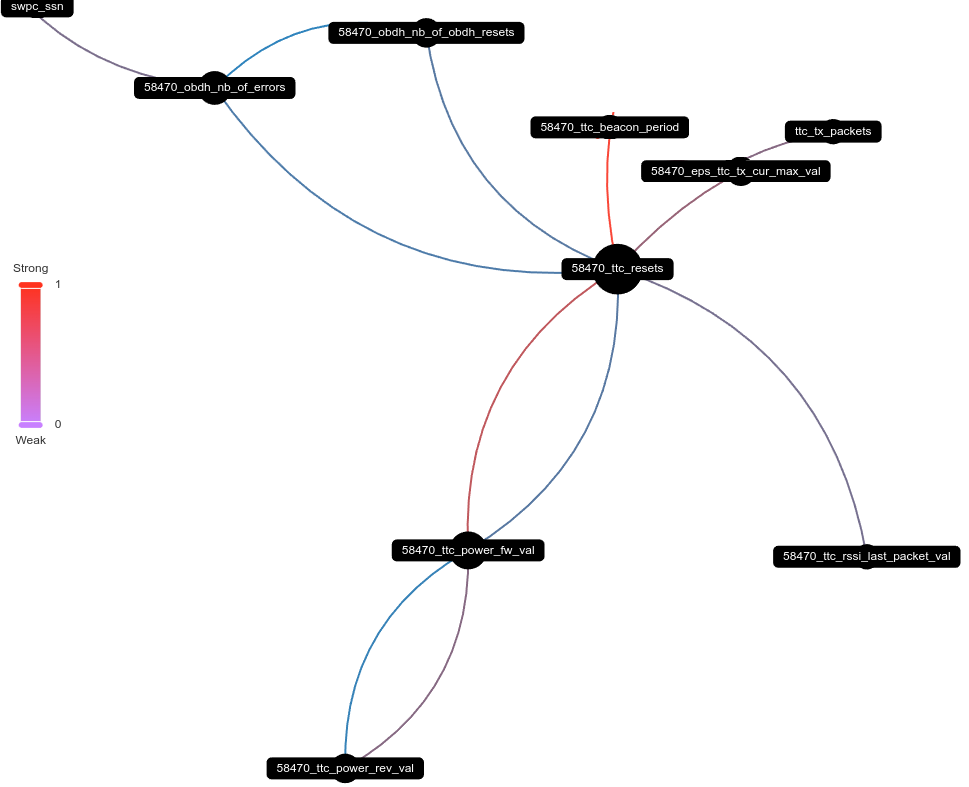
\includegraphics[width=0.95\textwidth]{sat/enso_ssn.png}
	\caption{Граф кросс-корреляций по числу солнечных пятен (ENSO)}
	\label{fig:enso_ssn}
\end{figure}

\begin{figure}[H]
	\centering
	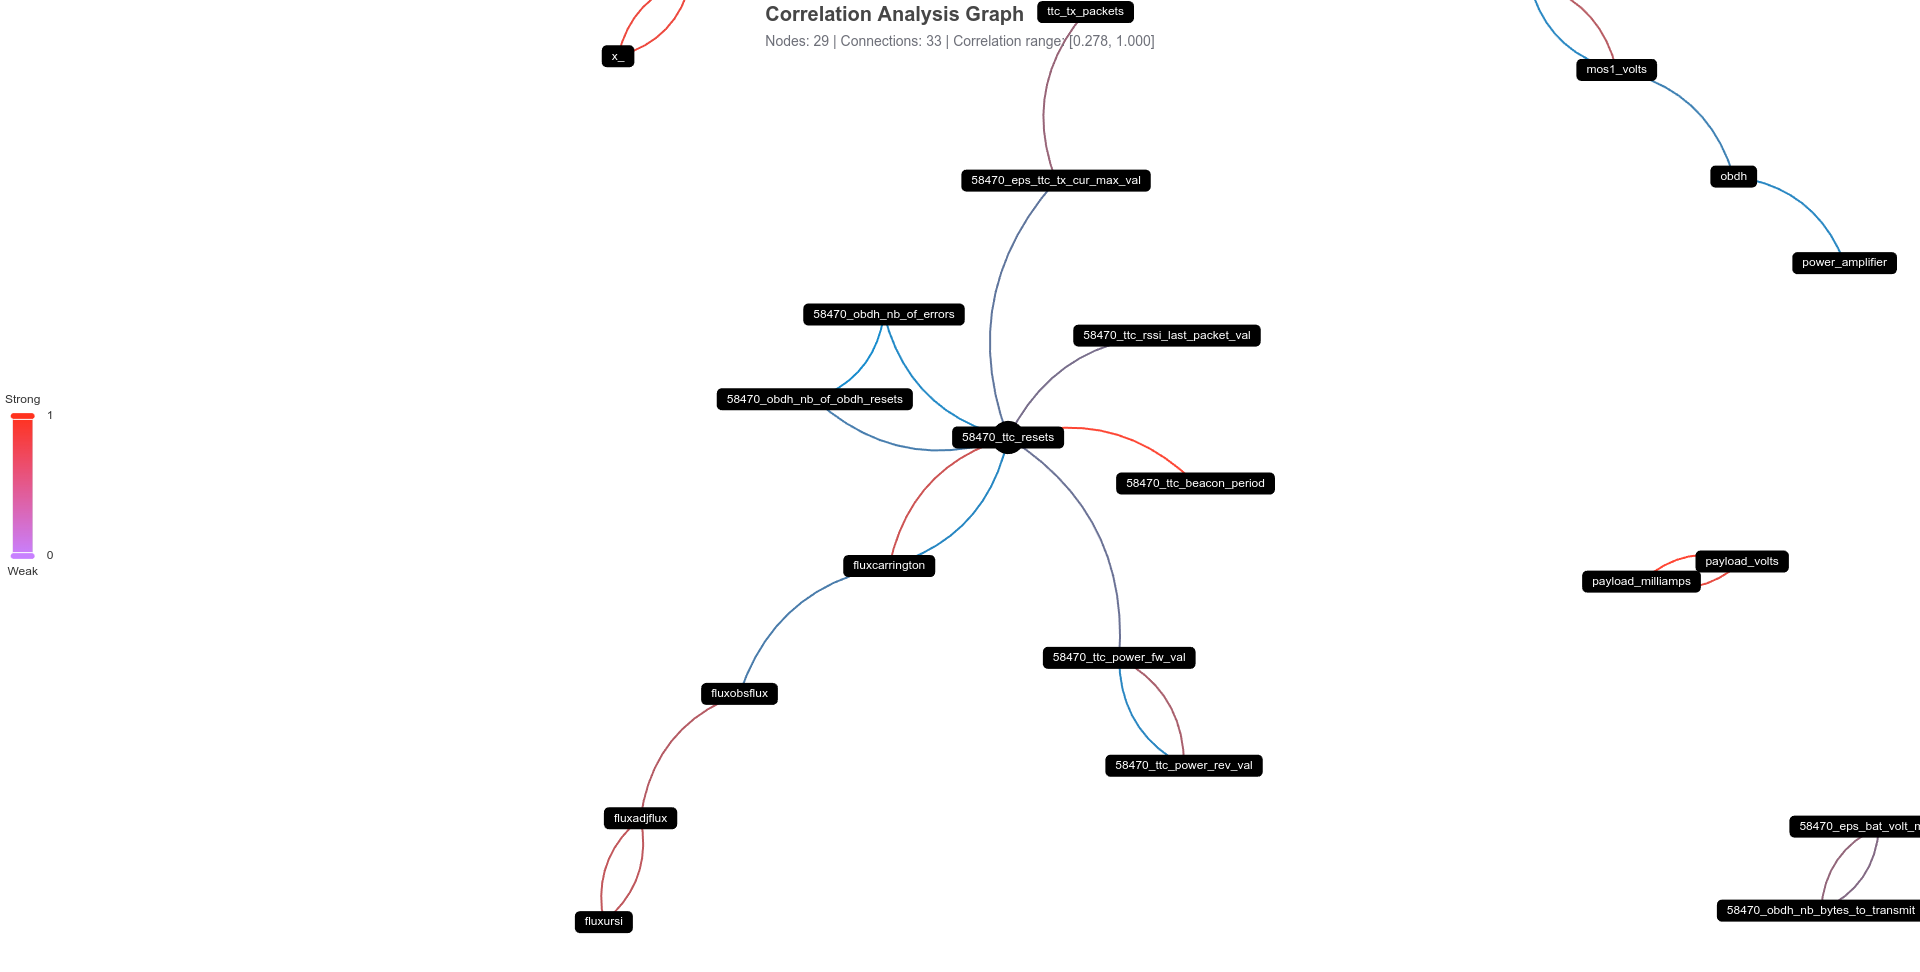
\includegraphics[width=0.95\textwidth]{sat/enso_flux.png}
	\caption{Граф кросс-корреляций по солнечному радиоизлучению (ENSO)}
	\label{fig:enso_flux}
\end{figure}

В центре большинства графов находится параметр \texttt{58470\_ttc\_resets} -
число перезапусков радиотехнического комплекса передачи данных. Этот параметр
тесно связан с ошибками и сбоями в подсистемах передачи и обработки информации
(\texttt{58470\_obdh\_nb\_of\_errors},
\texttt{58470\_obdh\_nb\_of\_obdh\_resets}), а также с энергетическими
характеристиками (\texttt{58470\_eps\_ttc\_bx\_cur\_max\_val},
\texttt{58470\_ttc\_power\_fw\_val}, \texttt{58470\_ttc\_power\_rev\_val}).

Анализ графа на рисунке~\ref{fig:enso_sunspot} показывает, что увеличение
количества ошибок и перезапусков в подсистемах (\texttt{obdh}, \texttt{ttc})
коррелирует с изменениями энергетических параметров. Связи между
\texttt{ttc\_resets} и \texttt{beacon\_period}, а также между
\texttt{ttc\_resets} и \texttt{ttc\_power\_fw/rev\_val} имеют различную силу:
наиболее сильные (красные рёбра) соответствуют случаям, когда сбои в питании или
перегрузки приводят к аварийным перезапускам радиотракта. Слабые (синие) и
средние (фиолетовые) связи фиксируют менее выраженные, но устойчивые зависимости
- например, рост тока передачи (\texttt{eps\_ttc\_bx\_cur\_max\_val}) при
увеличении числа пакетов (\texttt{ttc\_tx\_packets}), что отражает
закономерности работы CubeSat на низкой околоземной
орбите~\cite{expleo_enso_pdf}.

На графе~\ref{fig:enso_ssn} прослеживается связь между числом солнечных пятен
(\texttt{swpc\_ssn}) и инженерными параметрами. В периоды роста солнечной
активности наблюдается тенденция к снижению числа ошибок и перезапусков, что
связано с увеличением выработки энергии солнечными панелями и стабилизацией
работы энергетической подсистемы. Однако, при экстремальных событиях возможен
обратный эффект - рост числа сбоев из-за повышения радиационного
фона~\cite{nasa_shielding}.

Граф~\ref{fig:enso_flux} демонстрирует аналогичные закономерности для параметров
солнечного радиоизлучения (\texttt{fluxcarrington}, \texttt{fluxobsflux},
\texttt{fluxadjflux}, \texttt{fluxursi}). Сильные корреляции между током
нагрузки полезной нагрузки (\texttt{payload\_milliamps}) и напряжением
(\texttt{payload\_volts}) указывают на прямую зависимость между уровнем
солнечного излучения и энергетическими возможностями спутника. Связи между
параметрами питания и сбоями подтверждают, что энергетические провалы или
перегрузки приводят к увеличению числа перезапусков и ошибок в системах передачи
и обработки данных.

В периоды низкой солнечной активности возможно снижение напряжения и тока на
батареях (\texttt{eps\_bat\_volt\_avg\_val}, \texttt{battery\_voltage\_volts}),
что увеличивает риск сбоев и аварийных перезапусков. Это типично для малых
CubeSat, построенных на коммерческих компонентах без специализированной
радиационной защиты~\cite{expleo_enso_pdf, nanosats_enso}.

Таким образом, анализ графов кросс-корреляций для ENSO показывает, что ключевым
фактором надёжности работы спутника является энергетическая стабильность,
напрямую зависящая от солнечной активности. В периоды благоприятных условий
(высокая активность, стабильный поток излучения) количество сбоев и ошибок
минимально, а при экстремальных событиях или энергетическом дефиците -
возрастает.


\section{Структурный анализ графов кросс-корреляций и особенностей спутника Veronika}

\subsection{Структурные и технологические особенности спутника Veronika}

Veronika - это 1U CubeSat, разработанный и произведённый словацкой компанией Spacemanic при поддержке Deutsche Schule Bratislava, PLANETUM (Прага) и Технического университета Кошице~\cite{spacemanic_veronika, nanosats_veronika, satnogs_veronika, kozmonautika_veronika}. Аппарат был выведен на солнечно-синхронную орбиту высотой 550 км 11 ноября 2023 года ракетой Falcon 9 (миссия Transporter-9). Масса спутника составляет 1010 г, размеры - стандартный 1U форм-фактор.

Конструкция Veronika выполнена с использованием проверенных компонентов с богатой летной историей, разработанных и интегрированных компанией Spacemanic~\cite{spacemanic_veronika, nanosats_veronika}. Корпус изготовлен из анодированного алюминиевого сплава, что обеспечивает необходимую механическую прочность и минимальный уровень дегазации. Для электроизоляции и защиты от температурных перепадов применяются полиимидные материалы (например, Kapton), а для крепежа и кабельных соединений - стандартные полимерные материалы, используемые в индустрии малых спутников~\cite{spacemanic_veronika, kozmonautika_veronika}.

На борту установлены две камеры (uCAM и iCAM) для съёмки Земли, каждая из которых отличается компактностью, малой массой и низким энергопотреблением. uCAM - это малогабаритная камера с разрешением до 640×480, CMOS-сенсором и углом обзора 116°, а iCAM - более лёгкая камера с VGA-разрешением и углом обзора 60°~\cite{kozmonautika_veronika}.

Энергетическая подсистема включает солнечные панели и аккумуляторную батарею, обеспечивающие питание всех систем CubeSat. Радиокомплекс поддерживает работу в любительских диапазонах UHF (436.680 МГц) и VHF (145.925 МГц), реализованы протоколы AX.25, GFSK и CW для передачи телеметрии и пользовательских сообщений~\cite{spacemanic_veronika, nanosats_veronika, kozmonautika_veronika}. Важной особенностью является наличие экспериментальной системы ориентации (ADCS) с электромагнитными приводами и приёмником GNSS, что позволяет спутнику стабилизироваться и определять своё положение в пространстве~\cite{spacemanic_veronika, nanosats_veronika}.

Вся компонентная база - коммерческая (COTS), без применения специализированных радиационно-стойких решений, что типично для современных образовательных и технологических CubeSat~\cite{spacemanic_veronika, nanosats_veronika, nasa_soa}. Перед запуском Veronika прошла полный цикл испытаний на вибрацию, термовакуум и электромагнитную совместимость, что подтверждено инженерными отчётами компании~\cite{spacemanic_veronika, kozmonautika_veronika}.

\subsection{Анализ графов кросс-корреляций для спутника Veronika}

На рисунках~\ref{fig:veronika_sunspot}--\ref{fig:veronika_flux} представлены
графы кросс-корреляций между инженерными и внешними параметрами спутника
Veronika.

\begin{figure}[H]
	\centering
	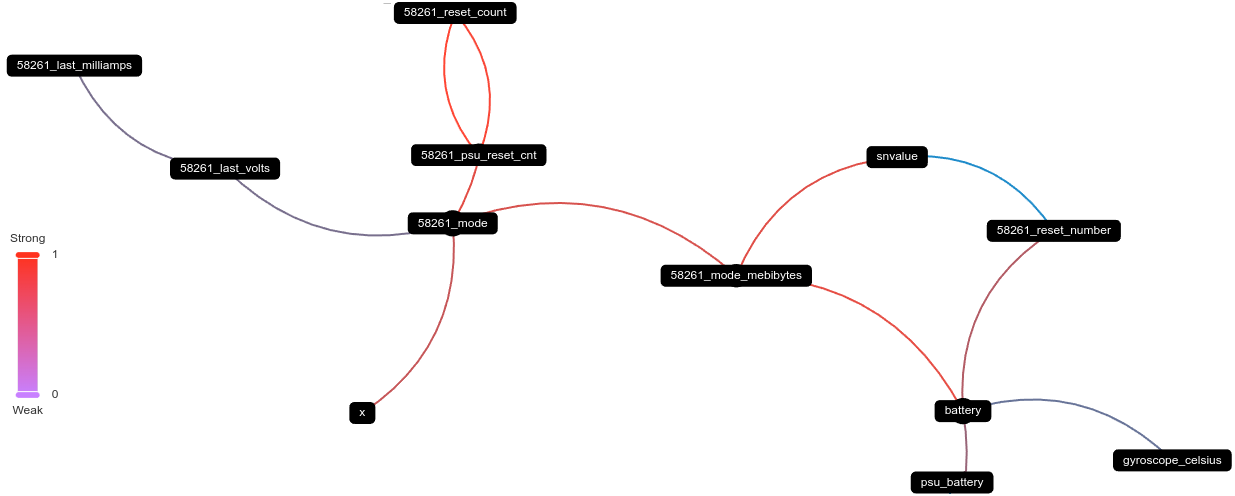
\includegraphics[width=0.95\textwidth]{sat/veronika_sunspot.png}
	\caption{Граф кросс-корреляций по инженерным параметрам и солнечным пятнам (Veronika)}
	\label{fig:veronika_sunspot}
\end{figure}

\begin{figure}[H]
	\centering
	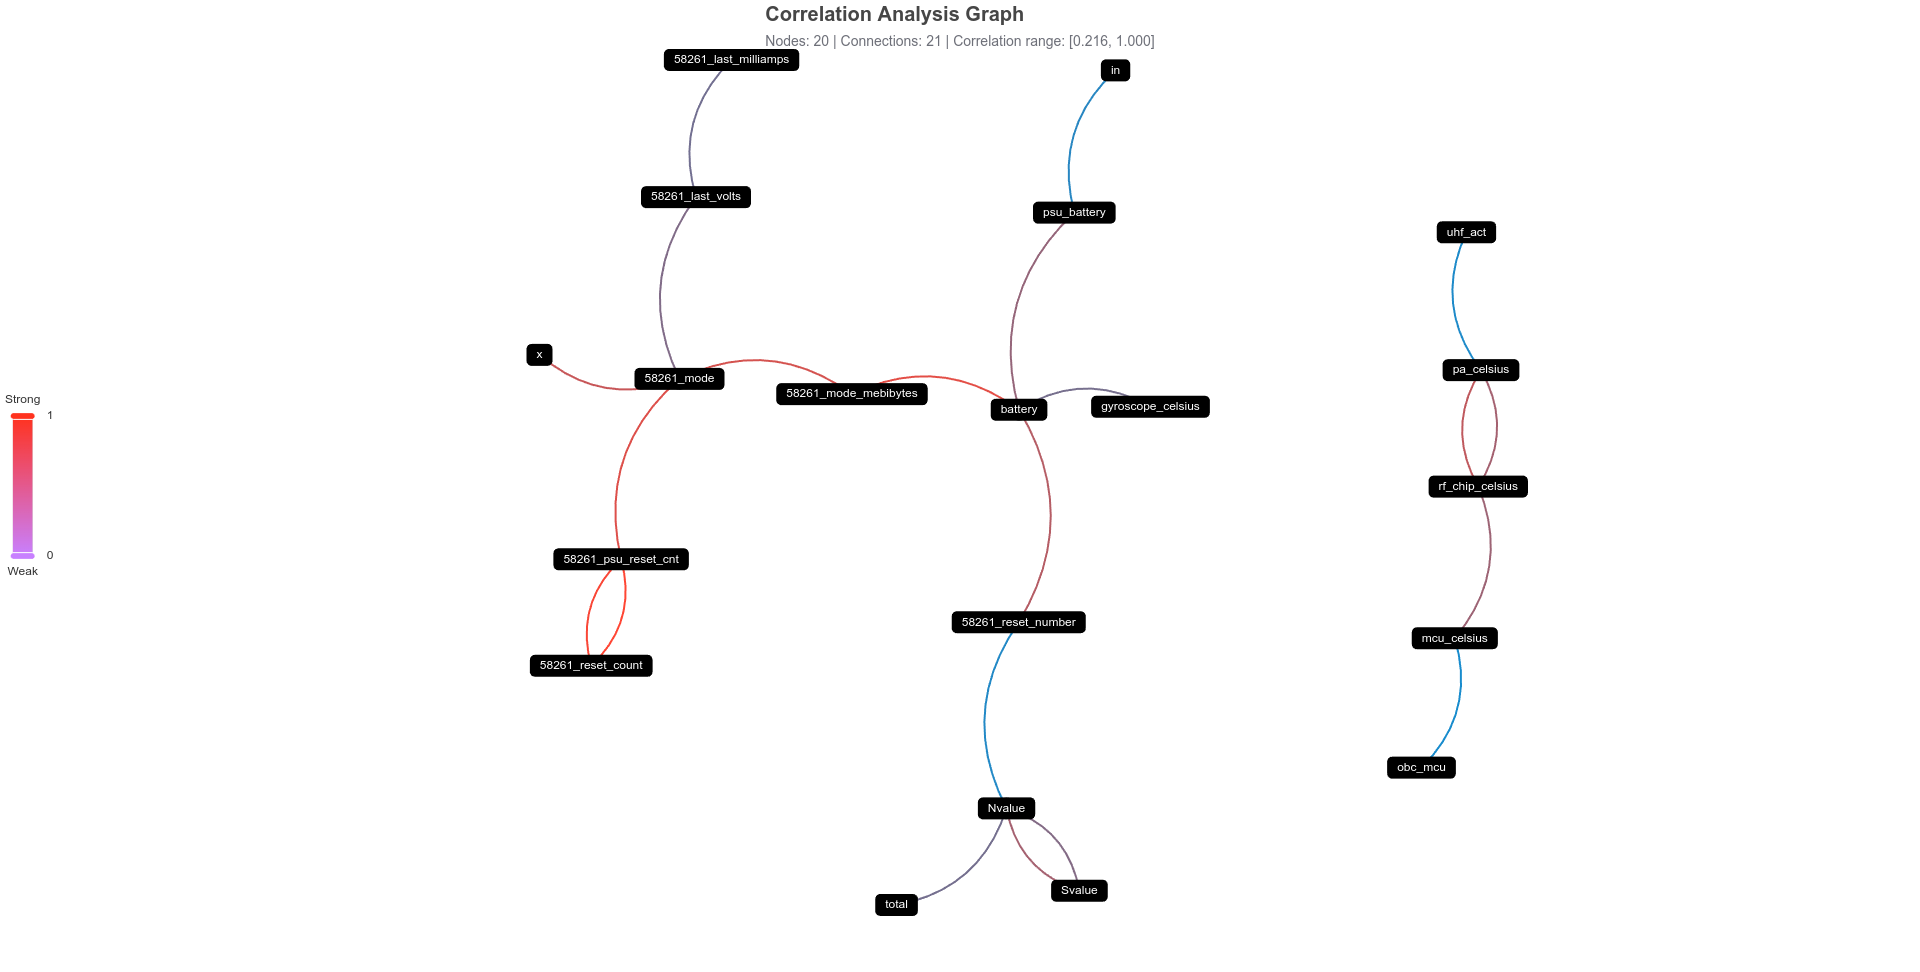
\includegraphics[width=0.95\textwidth]{sat/veronika_hemi.png}
	\caption{Граф кросс-корреляций по гемиcферическим числам солнечных пятен (Veronika)}
	\label{fig:veronika_hemi}
\end{figure}

\begin{figure}[H]
	\centering
	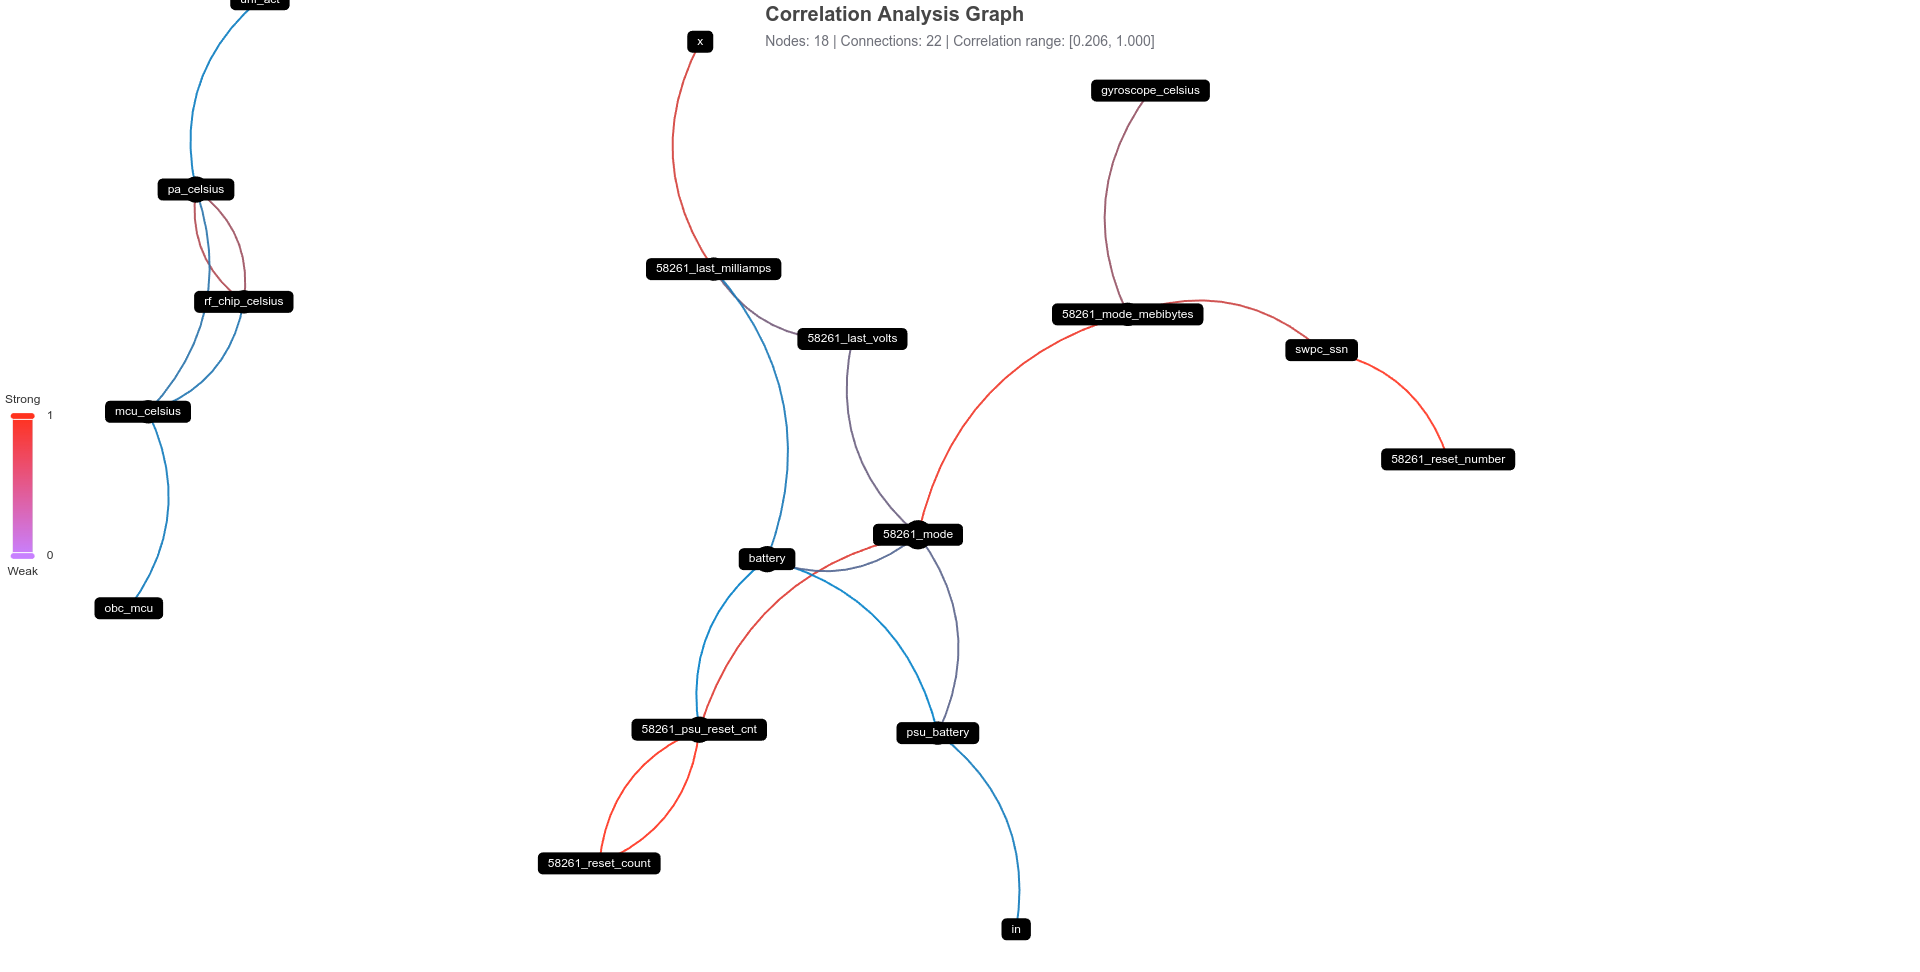
\includegraphics[width=0.95\textwidth]{sat/veronika_ssn.png}
	\caption{Граф кросс-корреляций по среднемесячному числу солнечных пятен (Veronika)}
	\label{fig:veronika_ssn}
\end{figure}

\begin{figure}[H]
	\centering
	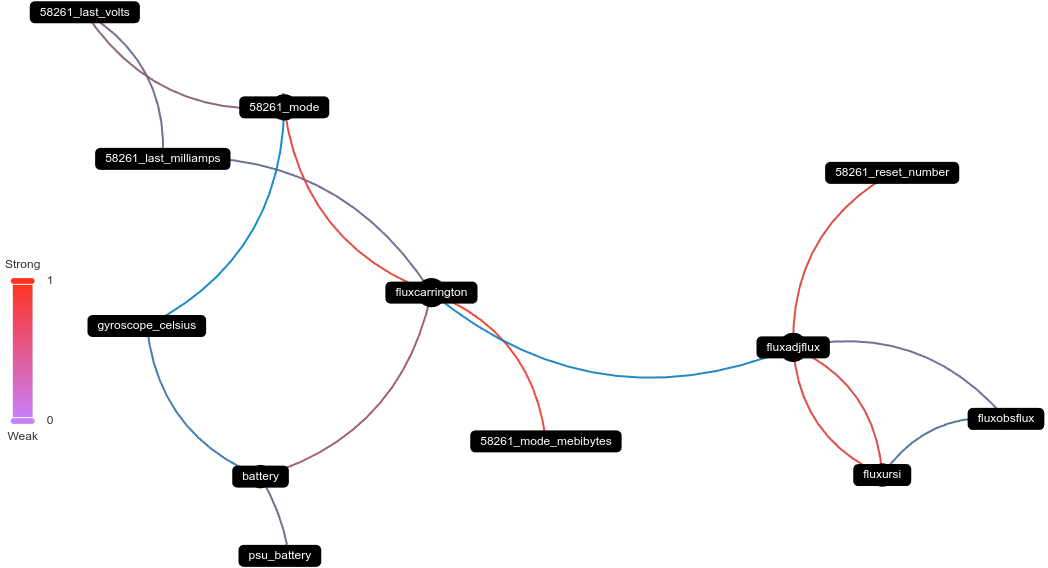
\includegraphics[width=0.95\textwidth]{sat/veronika_flux.png}
	\caption{Граф кросс-корреляций по солнечному радиоизлучению (Veronika)}
	\label{fig:veronika_flux}
\end{figure}


В центре представленных графов кросс-корреляций для спутника Veronika (рис.~\ref{fig:veronika_sunspot}--\ref{fig:veronika_flux}) находятся параметры, связанные не только с энергетикой, но и с логикой функционирования, сбоями и тепловыми режимами ключевых подсистем. Наиболее сильные корреляции (красные рёбра) фиксируются между счетчиками перезапусков (\texttt{58261\_reset\_count}, \texttt{58261\_psu\_reset\_cnt}, \texttt{58261\_reset\_number}) и рабочими режимами (\texttt{58261\_mode}, \texttt{58261\_mode\_mebbytes}), что указывает на прямую зависимость надёжности работы от переходов между режимами и состояния управляющей электроники. Это типично для малых спутников с ограниченными ресурсами: сбои часто инициируются не только энергетическими провалами, но и логическими ошибками, накоплением ошибок памяти или перегревом микроконтроллеров~\cite{spacemanic_veronika, nanosats_veronika}.

Графы демонстрируют, что влияние солнечной активности на Veronika не является однозначно положительным. С одной стороны, рост солнечной активности (параметры \texttt{swpc\_ssn}, \texttt{fluxcarrington}, \texttt{fluxobsflux}, \texttt{fluxadjflux}, \texttt{fluxursi}) приводит к увеличению выработки энергии солнечными панелями, что проявляется в корреляциях между током нагрузки (\texttt{58261\_last\_milliamps}), напряжением (\texttt{58261\_last\_volts}, \texttt{battery}, \texttt{psu\_battery}) и снижением числа аварийных перезапусков~\cite{spacemanic_veronika, nanosats_veronika}. Однако при экстремальных вспышках и магнитных бурях наблюдается усиление негативных эффектов: возрастает количество сбоев, увеличивается число аппаратных перезапусков, фиксируются скачки температур в чувствительных узлах (кластер температурных параметров: \texttt{mcu\_celsius}, \texttt{rf\_chip\_celsius}, \texttt{pa\_celsius}, \texttt{uhf\_act}, \texttt{obc\_mcu})~\cite{nasa_soa, stehlikova_veronika}.

Особо стоит отметить, что корреляции между температурными параметрами и сбоями не всегда линейны: перегрев радиотракта или управляющего микроконтроллера (\texttt{mcu\_celsius}, \texttt{rf\_chip\_celsius}) может быть как следствием интенсивной работы в условиях высокой солнечной активности, так и результатом внутренних сбоев, вызванных, например, ошибками в логике управления питанием. В ряде случаев наблюдается каскадный эффект: рост солнечной активности $\rightarrow$ увеличение выработки энергии $\rightarrow$ рост нагрузки на радиотракт $\rightarrow$ рост температуры $\rightarrow$ увеличение вероятности аппаратных сбоев и перезапусков~\cite{stehlikova_veronika, spacemanic_veronika}.

Связи между параметрами \texttt{battery}, \texttt{psu\_battery}, \texttt{last\_milliamps}, \texttt{last\_volts} и внешними индексами солнечной активности подтверждают, что энергетическая стабильность - лишь один из факторов надёжности. При недостатке солнечной энергии (низкая активность или затенение орбиты) риск сбоев увеличивается из-за разрядки батарей, однако при избыточной активности возможны перегревы и повреждения электроники, особенно в отсутствие специализированной радиационной и тепловой защиты, как у Veronika~\cite{spacemanic_veronika, stehlikova_veronika}.






